\documentclass{standalone}
\usepackage{tikz}
\usepackage{ctex,siunitx,bm}
\setCJKmainfont{Noto Serif CJK SC}
\usepackage{tkz-euclide,ninecolors}
\usepackage{amsmath}
\usetikzlibrary{patterns, calc}
\usetikzlibrary {decorations.pathmorphing, decorations.pathreplacing, decorations.shapes,}
\begin{document}
\small
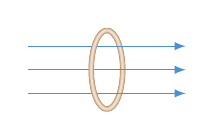
\begin{tikzpicture}[>=latex,yscale=1.0]
  \foreach \x in {80,60,40,20}
    {
      \draw[line width={2*sin(\x)},brown5!\x](0,0.5)arc(90:-90:0.2 and 0.5);
    }
  \foreach \x in {0.3,0,-0.3}
    {
      \draw[azure6,->](-1,\x)--(1,\x);
    }
  \foreach \x in {80,60,40,20}
    {
      \draw[line width={2*sin(\x)},brown5!\x](0,0.5)arc(90:270:0.2 and 0.5);
    }
\end{tikzpicture}
\end{document}